% Taken from outline.txt Section 3: VM support for DSU
%  Introduce them: reuse VM mechanisms
%    Class loading
%    On-line compilation
%    Thread sync (used for a full GC)
%    Copying GC traversal
%    On-stack replacement
%  Organize the structure of this section around these mechanisms
%    When describing each of these cases, use the running example to illustrate
%    Step 1: load and compile the new classes
%      renaming old classes, other gotchas
%    Step 2: wait for a safe point
%      Describe the safety condition
%        Distinguish the ideal condition from the one we actually use?
%         that is, if we supported on-stack replacement we could be
%         more liberal, right?
%       Implementation and implications to performance
%    Step 3: do the GC traversal
%      Explain how this works
%        Allocating space in new space for both old and new versions, etc.
%      Describe safety condition
%        The order of the traversal matters
%       Mention Boyapati stuff as the "right answer" to this problem
%       Indicate our simpler restriction
%         Cannot, transformer for A, look at the contents of fields of class B 
%            if class B has also changed
%           (this would be allowed if we knew B was encapsulated)
%       Indicate that this condition works fine for the updates we tried
%    Details
%      Say how many lines we had to change/add, etc.
%    Discussion: Performance
%      supporting inlining
%      supporting on-stack replacement
%  Discussion: Safety
%    Argument as to why our approach will yield type safety
%    Talk about issues with aliasing (along the lines of the long
%      conversation we had about Strings being turned into EmailAddresses
%      and how the programmer could ensure proper aliasing is preserved in
%      this case)

%       Mention Boyapati stuff as the "right answer" to this problem
%       Indicate our simpler restriction
%         Cannot, transformer for A, look at the contents of fields of class B 
%             if class B has also changed
%           (this would be allowed if we knew B was encapsulated)
%       Indicate that this condition works fine for the updates we tried
%     Details
%       Say how many lines we had to change/add, etc.
%     Discussion: Performance
%       supporting inlining
%       supporting on-stack replacement
%   Discussion: Safety
%     Argument as to why our approach will yield type safety
%     Talk about issues with aliasing (along the lines of the long
%       conversation we had about Strings being turned into EmailAddresses
%       and how the programmer could ensure proper aliasing is preserved in
%       this case)


\section{VM Support for DSU}
\label{sec:vm}

%% This section describes how existing modern virtual machine (VM)
%% services for managed languages are well suited to supporting dynamic
%% software updating. Specifically, it shows how to enhance existing
%% functionality in the VM's dynamic class loader, JIT compiler,
%% garbage collector, and scheduler to implement the update model
%% described above,

%% \DSU{} only applies updates at a VM \emph{yield point}.
%% Yield points are implemented as tests at method boundaries and loop
%% back edges at which the VM gains control of a thread. VMs need yield
%% points to safely perform thread scheduling, JIT recompilation, and
%% garbage collection.  


% Section 3: VM support for DSU
%   Introduce them: reuse VM mechanisms
%     Classloading
%     On-line compilation
%     Thread sync (used for a full GC)
%     Copying GC traversal
%     On-stack replacement


This section describes how we implement DSU by extending common
virtual machine services.  We
discuss our particular implementation choices in the context of
\JikesRVM{}~\cite{AAB+:99}, a high-performance~\cite{VMperf:webpage}
Java-in-Java Research VM\@. Our current \DSU{} implementation uses
\JikesRVM{}'s dynamic classloader, \acs{JIT} compiler, thread scheduler, and copying
garbage collector~\cite{BCM:04}.  Specifically, both \emph{class updates} and
\emph{method body updates} require VM
% \emph{method body updates} (see Section~\ref{sec:updates}), require VM
classloading, \acs{JIT} compilation, and thread scheduling support.
\emph{Class updates} additionally require garbage collection support.

After the user prepares and tests modifications and makes them available
for the update, the update process in \DSU{} proceeds in four steps.
First, a standalone tool prepares the update.  % When the update is
The user then signals \DSU{}, which waits until it is safe to apply the
update.  At this point \DSU{} stops running threads, and loads the
\suriya{might need some change}
updated classes, (we propose to perform this step asynchronously)
and installs the modified methods and classes.  Finally, if
needed, it performs a modified garbage collection that implements class
signature updates by transforming object instances from the old to the new
class definitions.

\subsection{\acf{UPT}}
\label{sec:prep}

To determine the changed and transitively-affected classes for a given
release, we wrote a simple \acf{UPT} that examines differences between
the old and new classes provided by the user.  \ac{UPT} is built on
top of
jclasslib,\footnote{\url{http://www.ej-technologies.com/products/jclasslib/overview.html}}
a bytecode viewer and library for examining (bytecode) class files.
\ac{UPT} first finds \emph{class updates} --- classes whose signatures
have changed due to field or method additions or deletions, or due to
method signature changes.  \ac{UPT} finds methods whose bodies have changed
and classifies them as \emph{method body updates}.  It simply compares
the bytecodes to make these classifications.
%
Finally, \ac{UPT} determines \emph{indirect method updates}, which are
methods whose source code is unchanged but refer to a field or method
in an updated class.  Such methods must be recompiled to correct field
or methods offsets that changed because of the update.  After an
update is loaded,
the VM also adds methods to this list similarly affected by its \acs{JIT} inlining choices.
\DSU{} does not load or compile indirectly-updated methods, but
rather invalidates the old compiled versions and the \acs{JIT} later
recompiles them on demand.

\suriya{Clarify how generates transformers}
As mentioned previously, \DSU{} generates the default transformer
internally.  In addition it provides
templates for object and class 
transformer functions, that the user may modify if necessary.
The user then presents the list of updated classes and user
transformers to \DSU{}.



\subsection{Stopping/Resuming Execution}
\label{sec:safe}

To preserve type safety, \DSU{} ensures that the update to the new
version is atomic.  No code from the new version must run before the
update completes, and no code from the old version must run afterward.
\DSU{} requires the running system to reach a \emph{DSU safe point}
before applying updates.  DSU safe points occur at \emph{VM safe
  points}, but further restrict the methods referenced by running
threads' stacks.  To safely perform VM services such as thread
scheduling, garbage collection, and \acs{JIT} compilation, \JikesRVM{} (like
most production VMs) inserts yield points at all method entry and exit
points, and loop back edges.  If the VM wants to perform a garbage
collection or schedule a higher priority thread, it sets a yield flag,
and the threads stop at the next VM safe point.  \DSU{} piggybacks on
this functionality.  When \DSU{} is informed an update is available,
it sets the yield flag.  Once all threads have reached VM safe points,
a DSU thread checks all thread stacks.  If none refers to a restricted
method, as defined below, the update is applied.  Otherwise, the
update is rejected, and must be retried. As part of proposed work, we
plan to implement a \DSU{} thread that wakes up periodically, and polls the
system to check if it is in a \emph{DSU safe point} and performs the
update.

\suriya{We have a timer retry. We
have to talk about this, when we have the right experiments.}

Similar to most other DSU
systems~\cite{ritzau00dynamic,Mala00a,altekar05opus,eaddy05enc,JVMhotswap,VSEnC,chen:icse07,K42reconfig},
\DSU's restricted methods include those belonging to classes that are
being updated.  To see why this restriction is important, consider the
update from Figure~\ref{fig:email-example} and assume the thread is
stopped at the beginning of the
\texttt{Configuration\-Manager.loadUser} method.  If the update takes
effect at this point, the implementation of
\texttt{User.set\-Forwarded\-Addresses} will take an object of type
\texttt{EmailAddress[]} as its argument.  However, if the old version
of \texttt{loadUser} were to resume, it would still call
\texttt{set\-Forwarded\-Addresses} with an array of \texttt{String}s,
resulting in a type error.

Preventing an update until updated methods are no longer on the stack 
ensures type safety because when the new version of the program resumes it
will be 
internally type correct.  If a 
programmer changes the type of a method \texttt{m}, for the program to
have compiled properly, the programmer must also change any methods that
call \texttt{m} to the new type.
In our example, the fact that \texttt{set\-For\-ward\-ed\-Ad\-dres\-ses}
changed type necessitated changing the function \texttt{loadUser} to
call it with the new type.  With this safety condition, there is no
possibility that the signature of method
\texttt{m} change and some old caller could call it---the update must also
include all callers of \texttt{m}.

However, restricting methods belonging to updated classes is not
enough---we must also restrict those methods updated indirectly %, i.e.,
% all methods identified by \ac{UPT}.  This is
because these methods
depend on the particular field and method offsets of the classes to
which they refer. If a class changes its signature, then its callers
must be recompiled to reflect that change.  Finally, we must also
restrict those methods into which updated methods---whether directly
or indirectly---have been inlined.  For example, if an updated method
\texttt{m} is inlined into another method \texttt{n}, then \texttt{n}
must also be considered restricted.  \DSU{} keeps track of the compiler's
inlining decisions and, when an update is available, computes a
transitive closure of all methods that have inlined methods
appearing in the update method set.  \DSU{} adds these additional
methods to the set of restricted methods used to determine a safe
point.

\paragraph{Discussion.}

While simple and largely efficacious, there are several possible
enhancements to our basic approach for establishing safe points.  

First, we could use
a static analysis to determine that some methods may be removed from
the restricted method set.  For example, Stoyle et al.'s static
analysis~\cite{StoyleHBSN06} would determine the update to \texttt{User}
could be permitted even while \texttt{loadUser} is running, but only
after the call to \texttt{setForwardedAddresses}.  Static analysis
however cannot enable updates to methods that are essentially
\emph{always} on the stack, such as infinite loops that perform event
processing.  Updates to methods containing such loops will be
indefinitely delayed.  To update in this case, past work has proposed
extracting out the contents of an infinite loop into separate methods
as a part of compiling updatable software, i.e., before the first
execution~\cite{neamtiu06dsu}.  Therefore, if the contents of the loop
change, the change is limited to the extracted method body, but the
loop itself and the type signature of the extracted method will remain
the same.  This source modification enables updates to the loop body
because there are windows in which it is not active, i.e., just before
or just after a call to the extracted method.
%
A similar technique could be implemented at update-time using \emph{on-stack
replacement}, which is provided in many VMs, including \JikesRVM{}.  The user would indicate the
correspondence between an infinite loop in the old version of the method and
the loop in the new version, and indicate how to map between the local
variables used in the two cases.

For the updates to programs we have considered, \DSU{} usually reaches
a safe point on the first try, as described
in Section~\ref{subsec:jetty}.  We have not explored retry
policies in any depth, but simple ones are obvious; e.g., retry the
update every $n$ milliseconds, or according 
to some distribution.  However, with a simple timer-based policy,
there may be but a small 
window in which the all forbidden methods are inactive, in which case
only a very lucky user will find that window.  A better approach would
be to delay an update, and use stack barriers~\cite{CHL:98} to
identify ripe conditions under which to try again.

A final possible enhancement is that the compiler could take care to
keep the field layout the same whenever possible, reducing the number
of updated methods and consequently the restricted method set.  We
leave exploration of these ideas to future work.


\paragraph{\acf{OSR}.}
\label{paragraph:osr}

By utilizing \acs{OSR}, we can push the envelope of active methods on stack
that \DSU{} allows during an update. \JikesRVM{}'s adaptive compiler
employs \acs{OSR} \cite{Fink:CGO:03} to transition from a long running
base-compiled version of a method to an optimized version. OSR
transformation involves the following three steps. 1) The VM extracts
compiler-independent state from the activation record of a suspended
thread. 2) The VM then generates specialized code for the suspended
activation. This code consists of a \emph{specialized prologue} that saves
values into locals and loads these values on the stack. 3) This specialized
code also transfers execution in the suspended thread to the optimized
version of the method at the current program counter.

\DSU{} can piggyback on OSR support to allow \emph{indirectly updated
methods} to be active on stack. The source code for these methods is
unchanged, but these methods must be recompiled because they refer to
offsets of fields or methods in updated classes. OSR needs no additional
information to recompile the method and jump to its new body.

To allow methods whose bodies are updated to be active on stack during the
update, \DSU{} must be able the compare their implementations to find a
correspondence between the old and updated versions, and identify the
method location to resume execution at after the update. This problem is in
general undecidable. We propose to implement an approach that we believe
will work in many cases. We propose to have \acs{UPT}, the offline tool
compare method implementations and provide \DSU{} a list of
methods and equivalent program execution points between the two versions,
that would let \DSU{} support updates to these methods.
% \DSU{} can use this list to support updates to these methods.
Also, a
method body change might add or remove local variables, and \DSU{} must
maintain a consistent stack mapping between the old and updated versions.
Moreover, these local variables might refer to objects whose classes are
updated and need to be transformed before the updated method can resume
execution.

\acs{OSR} in \JikesRVM{} and the extensions describes above only support
changes to the topmost method on the activation stack. We propose to use
stack barriers to support changes to other methods on stack. In order to
replace other methods on stack, we propose to overwrite the return address
of their activation records to jump to special barrier code. This code
examines the stack, uses \acs{OSR} to update the current method and returns
control back to the application. By maintaining the invariant that the
topmost method will always be of the new version, \DSU{} can update all
active methods on stack.



%  certain field layouts
% updated method may not 
% unnecessarily restrictive.  In particular, it could be that an updated
% class could be recompiled so as to not affect the method and field
% offsets of its existing members, in which cases clients would not have
% to be recompiled.  \mwh{Why was this hard to do?}

%% The challenge for on-stack replacement
%% is determining if there is a mapping from the old to the new
%% implementation.  In general, this problem is intractable, but for
%% narrowly scoped changes for example, changes limited to within a loop
%% nest it may be possible. In the context of a highly optimizing JIT
%% compiler, it would be very challenging to correlate the old optimized
%% code to the new implementation if the code has changed a lot.  

\subsection{Loading Modified Classes}

Once the program reaches a safe point, \DSU{} initiates the update.
There are two main steps in this process.  First, \DSU{}
loads the changed classes % and then arranges for them to be compiled
by adding metadata for new classes and updating %those for
the existing ones.
% properly by updating the metadata for the existing
% classes and adding metadata for new classes.
Second, the garbage
collector transforms existing object instances to refer to the new
metadata and, in the case of class signature changes, to use the new
object layout, initialized by the default or user-provided object
transformer function.  The remainder of this section covers the first
step, and the next subsection covers the second.

%% The Java language specification requires JVMs to perform dynamic
%% classloading. If the program references a class not currently
%% available in the VM, the VM must dynamically load it and either
%% compile it or interpret it.  \JikesRVM{} chooses to always compile to
%% the ISA of the underlying architecture.  This functionality easily
%% accommodates adding new classes---\DSU{} simply redirects the
%% classloader to the latest version of the method.


\begin{figure*}[t]
% \begin{center}
% \begin{tabular}{c|c|c}
% \scalebox{.7}{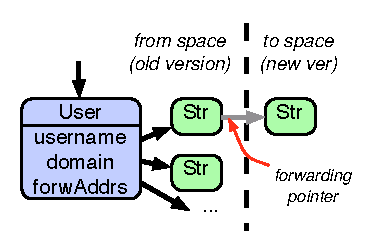
\includegraphics{gcupdate-simple1}} &
% \scalebox{.7}{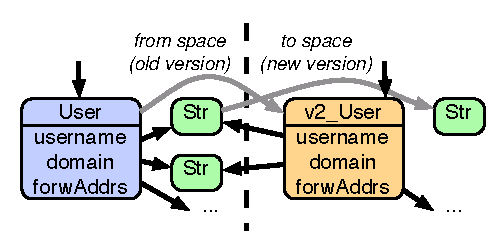
\includegraphics{gcupdate-simple2}} &
% \scalebox{.7}{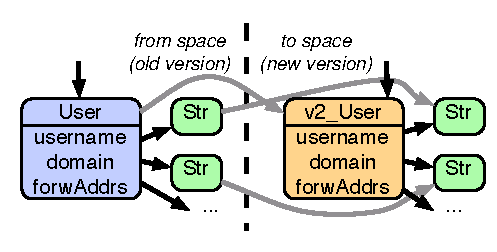
\includegraphics{gcupdate-simple3}} \\
% (i) before running transformer &
% (ii) after running transformer &
% (iii) GC+update complete \\
% \multicolumn{3}{c}{}\\
% \end{tabular}
% 
% (a) Running the default transformer during the GC
% \end{center}
% \hrule
\begin{center}
\scalebox{.7}{\includegraphics{gcupdate}}
% 
% (b) Running transformers following GC
\end{center}
\caption{Running object transformers following GC}
% \caption{Copying and transforming updated objects with the GC}
\label{fig:gc-example}
\end{figure*}

In \JikesRVM{}, a class has several data structures.
Each class has a corresponding \VMClass{} meta-object that describes
the class.  It points to other meta-objects that describe the class's
methods and fields, their types and offsets in an object instance.
% which describe the field or method's type, and its
% offset in an object instance.
The compiler uses offset information to
generate field and method access code, while the garbage collector
uses it to identify and trace object references.  % In addition to this metadata,
\VMClass{} also stores a \emph{type information block} (TIB) for each
class, which maps a method's offset to its actual implementation.
\JikesRVM{} chooses to always compile a method directly to machine code,
where the compilation takes place on-demand, when the method is first
called.  Each object instance
contains a pointer to its TIB, to support dynamic dispatch.  When the
program invokes a method on an object, the generated code
indexes the object's TIB at the correct offset and jumps to the
machine code.

For a class update, the class's number, type, and order of fields or
methods may have changed, which in turn impacts an object's layout and
its TIB.  To effect these changes, \DSU{} renames the old metadata for
the class (to eliminate name conflicts during object updates), and installs the new
\VMClass{} and corresponding metadata for the newly-compiled class.
Installing this information takes two steps.  First, the VM updates
several \JikesRVM{} data structures to indicate that the newly-loaded class
is now the up-to-date version.  These include the JTOC (Java Table of
Contents) for \texttt{static} methods and fields.  In addition, the VM
invalidates the TIB for all updated methods.  Just as with a
newly-loaded method, the \acs{JIT} will compile the updated method when it
is first invoked following the update.
The second step happens when the garbage collector traces objects
affected by the change: it updates them to point to their new TIB, as
well as applying their object transformer.

% Method body updates only change method code and not the class's
% layout, so \DSU{} overwrites the entries in the TIB of the existing
% class to point to the new method bodies, and discards the old method
% bodies.  All other meta-information about the class can remain
% unchanged.  As a result, existing object instances can be left
% alone---their TIB pointers and object layouts remain valid.

% As we pointed out in Section~\ref{sec:prep}, methods may have
% transitive dependences on others methods.  Since all highly optimizing
% JIT compilers perform inlining, they also introduce transitive
% dependences.  For example, if method \texttt{m} changes and it is inlined
% into another method, that method must also be recompiled.  In this
% first prototype implementation, we prevent the compiler from inlining.
% To support updates with inlining, \DSU{} needs the compiler to keep
% track of all its inlining decisions.  Then if a changed method has
% been inlined, \DSU{} will add that method to the list of methods to recompile
% and to the list of methods that must not be on the stack
% to safely perform the update. We expect to support inlining in the final
% version of the paper.

% Method signature updates are treated the same as class signature
% updates.  In these cases, the class' number, type, and order of
% fields or methods may have changed, which in turn impacts an object's
% layout and its TIB.  To effect these changes, \DSU{} renames the old
% metadata for the class (to use it during object updates), and installs
% the new \VMClass{} and corresponding metadata for the newly-compiled
% class.  Installing this information takes two steps.  First, several
% \JikesRVM{} data structures are updated to indicate that the newly-loaded
% class is now the up-to-date version.  These include the JTOC (Java
% Table of Contents) for \texttt{static} methods and fields.  Second,
% when the garbage collector traces objects affected by the change, it
% updates them to point to their new TIB as well as applying their
% object transformer.  We describe this process next.

% and
% points the TIB entry 

%% \suriya{jvolveclass. When we have class A \{ static String a =
%% "Hello"; \} who initializes A.a? javac generates a class initializer that
%% is called by the VM, and it does this. When a new field is introduced, we
%% cannot do that. I do not automatically generate the initializer. The
%% programmer has to initialize a new field explicitly in the jvolveclass
%% function}

%\mwh{below is Suriya's text.  Need to merge with my text above.}

%When a new version is available, \DSU{} must ensure that the update to a
%new version must happen atomically.  No code from the new version must run
%before the update, and no code from the old version must run after the
%update. All data structures must be conform to the new version after the
%update, both in terms of semantics and type-safety.

%\DSU{} uses a very simple non-deterministic approach to allow safe
%transformation to the new version. As mentioned earlier, the offline patch
%tool groups updates into those classes whose signatures have changed, and
%methods have to be recompiled either because they refer to these classes,
%or have changes to their method body.

% \DSU{} groups classes in the running program into the
% following groups: (a) Classes that have changed during the update. (b)
% Classes that contain methods that refer to fields and methods of classes in
% group A. These methods have to recompiled since their compiled code might
% refer to offsets that change after the update. Finally group (c), classes
% that are unaffected by this update.

%\DSU{} disallows any update that
%involves recompiling a function currently on stack either because it is a
%member of a classes in groups (a) or (b) as described above. When a new
%version is available, \DSU{} pauses all application threads, examines their
%stacks to see if the system is in safe state for the update to happen. If
%so, \DSU{} proceeds with the update, otherwise, \DSU{} resumes all threads,
%waits for a while before checking again.

%When the update happens, the stacks of all threads consist of methods that
%do not change in the new version. All classes from the old version that
%changed, are moved into a new namespace that is not accessed from any code
%in the new version. Any function call that is made is to code in the new
%version.

%The simple precondition that \DSU{} enforces is sufficient to
%ensure atomic updates. However, it is a bit too restrictive. We could
%utilize the VM's support for \ac{OSR} to support updates to methods on
%stack.

%\suriya{On stack replacement?}

%\subsection{Doing the update}
%When \DSU{} is ready to update, all application threads are paused, and the
%program is in a safe state. \DSU{} moves classes from the version that have
%been modified in the new version to a separate namespace. It then loads new
%versions of the updated classes. Loading the new class involves creating VM
%data structures to represent the new class such as a new \verb|VM_Class|
%object, a new Type Information Block (TIB), and new entries in the JTOC. At
%this point the classes from the new version have been added to the type
%hierarchy. For instance, as a result of modifying the classes Foo, Bar and
%Baz during the update, the class hierarchy would look like this:

%\begin{verbatim}
%Before:
%    Object
%    |-- Foo
%    `-- Bar
%        `-- Baz

%After:
%    Object
%    |-- Foo
%    |-- Bar
%    |   `-- Baz
%    |-- r2.Foo
%    `-- r2.Bar
%        `-- r2.Baz
%\end{verbatim}

%% \mwh{need to keep this text somewhere ...}

%% In order the build the new version with the update, we move the old version
%% into a separate package and compile this along with the new version. For
%% instance, 

%% \begin{verbatim}
%% === revision 3 ===
%% === Foo.java ===
%% class Foo {
%%     public static int x;
%% }
%% \end{verbatim}

%% \begin{verbatim}
%% === revision 4 ===
%% === r3/Foo.java ===
%% package r3;
%% class Foo {
%%     public static int x;
%% }

%% === Foo.java ===
%% import r3.*;
%% class Foo {
%%     public static int x;
%%     // y is precomputed to be factorial(x)
%%     public static int y;
%%     public static void
%%     type_transformer(r3.Foo from, Foo to) {
%%         to.x = from.x;
%%         to.y = factorial(to.x);
%%     }
%% }
%% \end{verbatim}

%   Organize the structure of this section around these mechanisms
%     When describing each of these cases, use the running example to illustrate
%     Step 1: load and compile the new classes
%       renaming old classes, other gotchas
%       Implementation and implications to performance
%     Step 3: do the GC traversal
%       Explain how this works
%         Allocating space in new space for both old and new versions, etc.
%       Describe safety condition
%         The order of the traversal matters

\subsection{Applying Transformers}
\label{sec:xformers}

%% We now need to convert objects to be of their updated types, and be
%% semantically consistent with the updated version of the application. The
%% type of each object is determined by the TIB pointed to by the object's
%% header. We need to change the type of objects by referring them to the new
%% TIBs. We also need to allocate additional space for new fields of the
%% object if necessary, and run the state transformation function to make the
%% object semantically consistent with the new version.

Existing objects whose class signatures have changed must be 
transformed via their object transformer methods.  We modify the \JikesRVM{}
semi-space copying collector \cite{BCM:04} to 
update changed objects as part of the collection, which is
safe because DSU safe points are a subset of GC safe points.  The VM
ensures that the stack maps are correct at every thread yield point.
Stack maps enumerate all registers, and stack variables that contain
root references in to the heap and are required to identifying reachable
objects.

A semi-space copying collector \cite{Cheney:70} normally works by traversing the
pointer graph in the heap (called \emph{from-space}) starting at the
roots and performing a transitive closure over the object graph, copying
all objects it encounters to a new heap (called \emph{to-space}).
Once the collector copies an object, it overwrites its header with a
forwarding pointer to the new copy in to-space.  If the collector
encounters the old object later during the traversal via another
reference, it uses the forwarding pointer to redirect the reference to
the new object.

Our modified collector works in much the same way, but differs in how
it handles objects whose class signature has changed.  In this case,
it allocates a copy of the old object \emph{and} a new object of the new
class (which may be a different size compared to the old one). The collector
initializes the new object to point to the TIB of the new type, and
installs a forwarding pointer in from-space to this new version. Next,
the collector stores a pair of pointers, one to the copy of the old object and one to the
new object in an update log.  The collector continues scanning the
copy of the old version.  After the collection completes, \DSU{} goes
through the update log and invokes the relevant object transformer
(either the default, or the user provided \texttt{jvolve\_object}), passing
the old and new object pairs as arguments.  Once all
pairs have been processed, the log is deleted, making the  duplicate
old versions unreachable. They will be reclaimed by the next collection.
Finally, \DSU{} executes the class transformers.

Figure~\ref{fig:gc-example} illustrates a part of the heap at the end
of the GC phase while applying the update from
Figure~\ref{fig:example-xform} (forwarding pointers are not shown to
avoid clutter).  On the left is a depiction of part of the heap prior
to the update.  It shows a \texttt{User} object whose fields point to
various other elided objects.  After the copying phase, all of the old
reachable objects have been duplicated in to-space.  The
transformation log points to the new version of \texttt{User} (which
is initially empty) and the duplicate of the old version, both of
which are in to-space.  The transformer function can safely copy
fields of the \texttt{from} object. The figure shows that after
running the transformer function, the new version of the object points
to the same \texttt{username} field as before, and it points to a new
array which points to new \texttt{EmailAddress} objects. The
constructor initialized these objects by referring to the old e-mail
\texttt{String} values and assigning fields to point to substrings of
the given \texttt{String}.

In our example, the \texttt{jvolve\_object} function only copies the
contents of old \texttt{User} objects' fields.  More generally,
the fields of old objects can
be dereferenced safely so long as all objects they point to are
up-to-date.  If one of the fields points to an object whose class has
been updated, it is possible that the pointed-to object has not yet
been transformed (i.e., since it appears later in the update log).  To
transform it, we could find the old object by scanning the remainder
of the update log and then pass both old and new objects to the
\texttt{jvolve\_object} method (or the default transformer).
To avoid multiple scans of the update log, we instead cache a pointer to
the old version from 
its new version when performing the GC (this pointer is not shown in
the figure).

We must also take care that \texttt{jvolve\_object} functions invoked
recursively to transform old objects do not loop infinitely (which would
constitute one or more ill-defined transformer functions). We detect
cycles with a simple check, and abort the update if a cycle is found.
In our current implementation, the programmer indicates whether to
transform a child object before or after the parent at the start of
the \texttt{jvolve\_object} function.  It should be straightforward to
determine when this case automatically, through a read barrier during
collection in the \texttt{jvolve\_object} code, or even simple
analysis of the \texttt{jvolve\_object} bytecode.
\suriya{Need to explain this better. Talk about "safety". Also, races in
transformation functions.}

Our approach of requiring an extra copy of all updated objects adds
temporary memory pressure, since copies will persist until the next GC\@.
Instead, we propose to copy the old versions to a special block of memory
that can be reclaimed after the collection completes.

\paragraph{Transforming objects within a concurrent garbage collector.}
\DSU{}'s current design requires a stop-the-world garbage collector that
requires the application to pause for the duration of a full GC\@.
Applications with real-time requirements use concurrent garbage collectors
where the collector runs concurrently with the application, to limit pause
times. Concurrent
collectors use read and write barriers to prevent the application from
disrupting the tricolor abstraction maintained by the collector. \DSU{}
must piggyback on top of these barriers to lazily transform objects as
they are needed. In Baker's algorithm \cite{Baker:1978}, when the
application encounters an object in \emph{from space}, it triggers the read
barrier code which copies the object to \emph{to space}. \DSU{}, when using
such a collector, in addition to copying them must lazily transform objects
from the old version when encountering them. Variations on Baker such as
Brooks \cite{Brooks:1984} and Appel-Ellis-Li collectors \cite{Appel:1988} all follow the same
principle but make various optimizations to the read-barrier code. We
propose to explore mechanisms and costs of supporting supporting DSU with
concurrent collectors.
% the costs of read barriers in concurrent collectors for
% DSU.
% Huelsbergen and Larus distinguish between mutable and immutable data, and
% use this opportunity to reduce the cost of accessing immutable data.
% Immutable 
% barriers \cite{Appel
Lazily applying object transformers has been explored
before~\cite{ritzau00dynamic,Mala00a,neamtiu06dsu,chen:icse07}.  The
main drawback here is that code must be inserted to check, at each
dereference, whether the object is up-to-date, imposing extra overhead
on normal execution.  Moreover, stateful actions by the program after
an update may invalidate assumptions made by object transformer
functions.  It is possible that a hybrid solution could be adopted,
similar to Chen et al.~\cite{chen:icse07}, which removes checking
code once all objects have been updated.

% We could attempt to avoid
% extra copying altogether by invoking object 
% transformer functions during collection.  This approach is more
% complicated because it may require recursively invoking the collector
% from the transformer if a dereferenced field has not yet been
% processed.  We also would need to insert an extra GC-time read barrier
% that follows forwarding pointers before dereferencing an object, and
% that determines whether an object has been transformed yet.  We leave
% exploration of these ideas to future work.

% We use a stop-the-world garbage collection-based approach
% that requires the application to pause for the
% duration of a full GC\@.  This pause time could be mitigated by
% piggybacking on top of a concurrent,
% collector.  We could also consider applying object and 
% class transformers lazily, as they are
% needed~\cite{ritzau00dynamic,Mala00a,neamtiu06dsu,chen:icse07}.  The
% main drawback here is that code must be inserted to check, at each
% dereference, whether the object is up-to-date, imposing extra overhead
% on normal execution.  Moreover, stateful actions by the program after
% an update may invalidate assumptions made by object transformer
% functions.  It is possible that a hybrid solution could be adopted,
% similar to Chen et al.~\cite{chen:icse07}, which removes checking
% code once all objects have been updated.

% In addition, to provide access to the fields 
% of changed objects in transformer functions, we can customize the
% collector to completely process the children first using a postorder
% traversal.  This traversal order would guarantee that any object
% reachable from the object transformer function is sure already initialized.
% Other programming 
% interfaces are possible, too.  For example, Boyapati et al.~\cite{boyapati03lazy}
% take advantage of encapsulation information to allow transformer code
% to access the old versions of pointed-to objects.  Our approach allows
% programs to only see the new versions of objects within transformers,
% similar to the \emph{representation consistency} invariant proposed by
% Stoyle et al.~\cite{StoyleHBSN06}.  We will let future experience
% guide our understanding of which programming interfaces are most
% useful.

% These disadvantages have not proved problematic in practice.  Very often the
% default transformer is sufficient, in which case there is no extra copying.
% The custom object transformer functions we have written are similar to the
% one in Figure~\ref{fig:example-xform}.  By and large, they copy fields
% (either base types or pointers) from the old object to the new one.
% Transformers also tend to allocate new objects for changed or added fields,
% and these new objects may, once again, refer to objects directly pointed to
% by the old object.  In the figure, the new \texttt{EmailAddress} objects
% point to the \texttt{String}s that used to serve as e-mail addresses in the
% old object.

% We use a stop-the-world garbage collection-based approach
% that requires the application to pause for the
% duration of a full GC\@.  This pause time could be mitigated by
% piggybacking on top of a concurrent,
% collector.  We could also consider applying object and 
% class transformers lazily, as they are
% needed~\cite{ritzau00dynamic,Mala00a,neamtiu06dsu,chen:icse07}.  The
% main drawback here is that code must be inserted to check, at each
% dereference, whether the object is up-to-date, imposing extra overhead
% on normal execution.  Moreover, stateful actions by the program after
% an update may invalidate assumptions made by object transformer
% functions.  It is possible that a hybrid solution could be adopted,
% similar to Chen et al.~\cite{chen:icse07}, which removes checking
% code once all objects have been updated.




% vim:spell:ft=tex:
